\documentclass[a4paper]{article}

% Packages
\usepackage[14pt]{extsizes}
\usepackage[T2A]{fontenc}
\usepackage[russian]{babel}
\usepackage[left=20mm, top=15mm, right=15mm, bottom=20mm]{geometry}
\usepackage{graphicx} % For images
\usepackage{amsmath, amssymb} % For equations
\usepackage{booktabs} % For better tables
\usepackage{pgfplots} % For plotting graphs
\usepackage{xcolor} % For color support
\usepackage{caption} % For captioning tables and figures
\usepackage{float} % For precise float placement (images, tables)
\usepackage{array} % For better table management
\pgfplotsset{compat=1.17}

% Importing custom definitions (lstset, tikzset, etc.)
\newcommand{\labtitle}[9]{
	\begin{center}
		\vspace*{-1.8cm}
		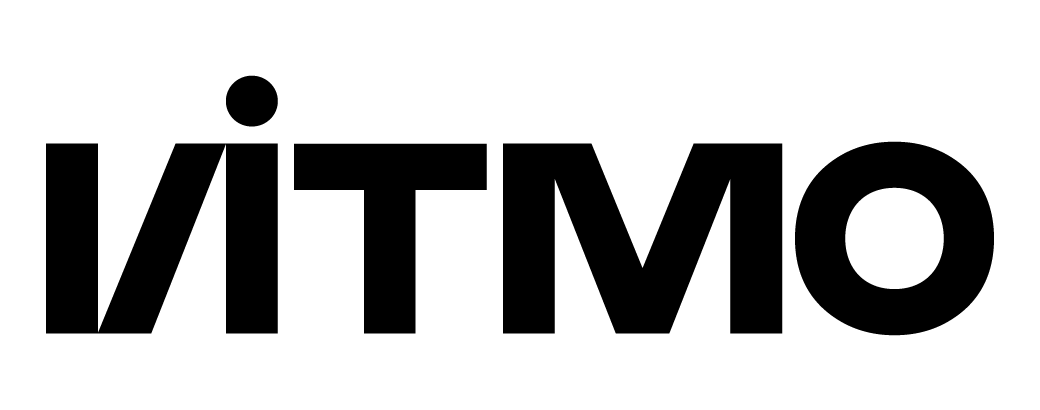
\includegraphics[width=0.26\textwidth]{../common/itmo-logo.png}\\
		\vspace{2.4cm}
		\textbf{\Large Основы электротехники}\\[1.2cm]
		\textbf{\Large Отчёт по лабораторной работе №#1}\\[0.7cm]
		\textbf{\Large #2}\\[3cm]

		\textbf{\Large Группа \textcolor{red}{\textit{P#3}}}\\[0.2cm]
		\textbf{\Large Вариант \textcolor{red}{\textit{#4}}}\\[3cm]

		\begin{flushleft}
			\textbf{\large Выполнил: \textcolor{red}{\textit{#5}}}\\[0.5cm]
			\textbf{\large Дата сдачи отчёта: \textcolor{red}{#6}}\\[0.5cm]
			\textbf{\large Дата защиты: \textcolor{red}{#7}}\\[0.5cm]
			\textbf{\large Контрольный срок защиты: \uline{#8}}\\[0.5cm]
			\textbf{\large Количество баллов: \uline{#9}}\\[2cm]
		\end{flushleft}
	\end{center}

	\vspace*{\fill}
	\begin{center}
		\textbf{\Large СПб -- 2024}
	\end{center}
	\vspace*{-1.8cm}
}

\newcommand{\hwtitle}[8]{
	\begin{center}
		\vspace*{-1.8cm}
		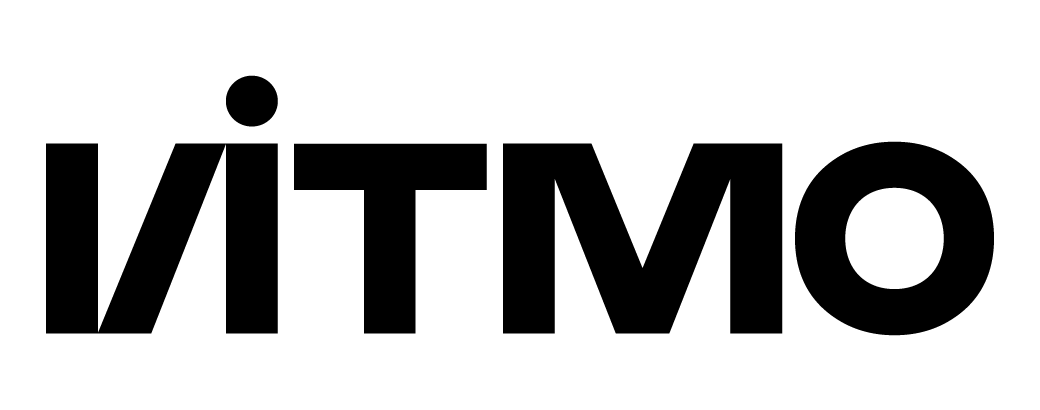
\includegraphics[width=0.26\textwidth]{../common/itmo-logo.png}\\
		\vspace{2.4cm}
		\textbf{\Large Основы электротехники}\\[1.2cm]
		\textbf{\Large Домашнее задание №#1}\\[0.7cm]
		\textbf{\Large #2}\\[3cm]

		\textbf{\Large Группа \textcolor{red}{\textit{P#3}}}\\[0.2cm]
		\textbf{\Large Вариант \textcolor{red}{\textit{#4}}}\\[3cm]

		\begin{flushleft}
			\textbf{\large Выполнил: \textcolor{red}{\textit{#5}}}\\[0.5cm]
			\textbf{\large Дата сдачи: \textcolor{red}{#6}}\\[0.5cm]
			\textbf{\large Контрольный срок сдачи: \uline{#7}}\\[0.5cm]
			\textbf{\large Количество баллов: \uline{#8}}\\[2cm]
		\end{flushleft}
	\end{center}

	\vspace*{\fill}
	\begin{center}
		\textbf{\Large СПб -- 2024}
	\end{center}
	\vspace*{-1.8cm}
}

% % listing for programming code blocks
\lstset{
	language=C++,                 % Programming language
	basicstyle=\ttfamily\normalsize, % Adjust font size
	keywordstyle=\color{blue},    % Style for keywords
	stringstyle=\color{red},      % Style for strings
	commentstyle=\color{gray},   % Style for comments
	morecomment=[l][\color{magenta}]{\#}, % Special comment style
	breaklines=true,              % Line breaking in long lines
	numbers=left,                 % Line numbering on the left
	numberstyle=\tiny\color{gray},% Style for line numbers
	frame=single,                 % Code frame
	showstringspaces=false        % Don't show spaces in strings
}

% % tikz styles for flowcharts
\tikzset{
	startstop/.style={
			rectangle,
			rounded corners,
			minimum width=3cm,
			minimum height=1cm,
			text centered,
			draw=black,
			fill=red!30
		},
	io/.style={
			trapezium,
			trapezium left angle=70,
			trapezium right angle=110,
			minimum width=3cm,
			minimum height=1cm,
			text centered,
			draw=black,
			fill=blue!30
		},
	process/.style={
			rectangle,
			minimum width=3cm,
			minimum height=1cm,
			text centered,
			draw=black,
			fill=orange!30
		},
	decision/.style={
			diamond,
			aspect=2,
			minimum width=3cm,
			text centered,
			draw=black,
			fill=green!30
		},
	arrow/.style={
			thick,
			->,
			>=stealth
		},
	prep/.style={
			chamfered rectangle,
			chamfered rectangle xsep=2cm,
			draw,
			thick,
			minimum width=5cm,
			minimum height=1cm,
			text centered,
			text width=2.5cm,
			font=\small,
			fill=yellow!30
		},
}


\begin{document}

% Title page
\labtitle{1}{Исследование характеристик источника электрической энергии постоянного тока}{3331}{33}{Дворкин Борис Александрович}{11.09.2024}{18.09.2024}{09.10.2024}{}
\thispagestyle{empty}

\newpage
\pagestyle{plain}
\setcounter{page}{1}

% Section 1: Схема эксперимента
\section{Схема эксперимента}
На рисунке 1.1 представлена схема замещения источника электрической энергии постоянного тока и нагрузки, созданная в приложении LTspice.

\begin{figure}[H]
	\centering
	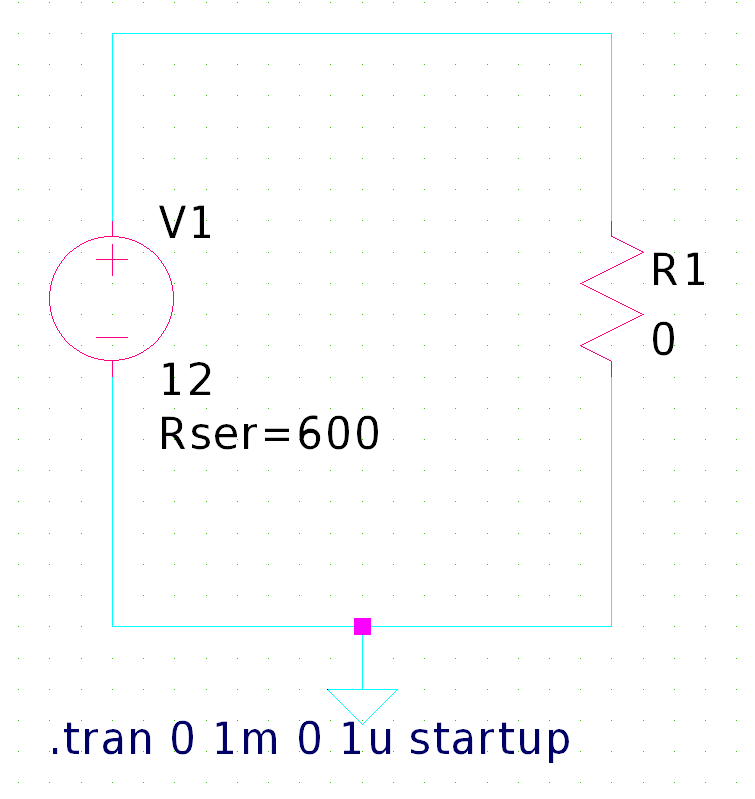
\includegraphics[width=0.6\textwidth]{schema.png} % Make sure the path to the image is correct
	\caption{Схема замещения источника электрической энергии в LTspice.}
\end{figure}

% Section 2: Таблица измерений
\section{Заполненная таблица 1.1}
\begin{table}[H]
	\centering
	\addtocounter{table}{0}
	\caption*{Таблица 1.1: Результаты измерений и расчётов}
	\begin{tabular}{|c|c|c|c|c|c|c|}
		\hline
		k  & \multicolumn{2}{c|}{Измерения} & \multicolumn{4}{c|}{Расчёт: r = 594.208 [Ом], E = 12 [B], Isc = 20 [мА]}                                            \\
		\hline
		0  & $R_n$ [Ом]                     & $U_n$ [В]                                                                & $I_n$ [мА] & $P_n$ [Вт] & $n$ & $r$ [Ом] \\
		\hline
		1  & $\infty$                       & 12.000                                                                   & 0.00       & 0.00       & 1.0 & --       \\
		2  & 5400                           & 10.692                                                                   & 1.98       & 0.021      & 0.9 & 600.00   \\
		3  & 2400                           & 9.504                                                                    & 3.96       & 0.038      & 0.8 & 600.00   \\
		4  & 1400                           & 8.316                                                                    & 5.94       & 0.049      & 0.7 & 600.00   \\
		5  & 900                            & 7.128                                                                    & 7.92       & 0.056      & 0.6 & 600.00   \\
		6  & 600                            & 5.940                                                                    & 9.9        & 0.059      & 0.5 & 600.00   \\
		7  & 400                            & 4.752                                                                    & 11.88      & 0.056      & 0.4 & 599.294  \\
		8  & 257                            & 3.563                                                                    & 13.864     & 0.049      & 0.3 & 600.709  \\
		9  & 150                            & 2.376                                                                    & 15.84      & 0.038      & 0.2 & 601.729  \\
		10 & 67                             & 1.193                                                                    & 17.806     & 0.021      & 0.1 & 543.756  \\
		11 & 0                              & 0.000                                                                    & 20         & 0.000      & 0.0 & --       \\
		\hline
	\end{tabular}
\end{table}

% Section 3: Пример расчёта
\newpage
\section{Пример расчёта для одной строки таблицы}

Для расчёта параметров используем следующие формулы:

\begin{itemize}
	\item Ток через нагрузку:
	      \[
		      I_n = \frac{U_n}{R_n}
	      \]

	\item Мощность, рассеиваемая на нагрузке:
	      \[
		      P_n = \frac{U_n^2}{R_n}
	      \]

	\item Коэффициент полезного действия:
	      \[
		      \eta_n = \frac{R_n}{R_n + r}
	      \]

	\item Внутреннее сопротивление источника:
	      \[
		      r_k = \frac{U_k - U_{k+1}}{I_{k+1} - I_k}
	      \]
\end{itemize}

Рассчитаем значения для строки \(n = 2\):

\begin{align*}
	I_2    & = \frac{U_2}{R_2} = \frac{10.692}{5400} = 1.98 \, \text{мА},                           \\
	P_2    & = \frac{U_2^2}{R_2} = \frac{10.692^2}{5400} \approx 0.021 \, \text{Вт},                \\
	\eta_2 & = \frac{R_2}{R_2 + r} = \frac{5400}{5400 + 600} = 0.9,                                 \\
	r_2    & = \frac{U_2 - U_3}{I_3 - I_2} = \frac{10.692 - 9.504}{3.96 - 1.98} = 600 \, \text{Ом}.
\end{align*}

Таким образом, для строки \(n = 2\) были рассчитаны следующие значения:
\[
	I_2 = 1.98 \, \text{мА}, \quad P_2 = 0.021 \, \text{Вт}, \quad \eta_2 = 0.9, \quad r_2 = 600 \, \text{Ом}.
\]


% Section 4: Расчётная внешняя характеристика источника
\newpage
\section{Расчётная внешняя характеристика источника}

На рисунке \ref{fig:characteristic} представлена расчётная и экспериментальная внешняя характеристика источника.
Расчётная характеристика изображена в виде синей линии,
которая соединяет точки \((0, E = 12 \, \text{В})\) и \((I_{sc} = 20 \, \text{мА}, 0)\).
Эта линия отражает теоретическую зависимость напряжения на нагрузке \(U_n\) от тока \(I_n\),
поступающего от источника, при идеальных условиях.

Экспериментальные точки, отмеченные на графике красными квадратами,
соответствуют измеренным значениям напряжения \(U_n\) для разных токов \(I_n\),
согласно данным из таблицы 1.1. Эти точки показывают реальные данные,
полученные при изменении сопротивления нагрузки, и их отклонения от расчётной линии
могут свидетельствовать о наличии потерь или неточностей в измерениях и/или вычислениях.

\begin{figure}[h]
	\centering
	\begin{tikzpicture}
		\begin{axis}[
				width=17cm, height=14cm, % Размер графика
				xlabel={$I_n$ [мА]}, % Ось X
				ylabel={$U_n$ [В]},  % Ось Y
				axis lines=middle,
				grid=major,          % Основная сетка
				xmin=0, xmax=22,     % Диапазон по оси X
				ymin=0, ymax=13,     % Диапазон по оси Y
				domain=0:20,         % Область построения
				thick,               % Толщина линии
				legend style={at={(0.95,0.95)}, anchor=north east}, % Легенда
				label style={font=\small},
				tick label style={font=\small},
				xtick={0, 2.5, 5, 7.5, 10, 12.5, 15, 17.5, 20}, % Подписи по оси X
				ytick={0, 1, 2, 3, 4, 5, 6, 7, 8, 9, 10, 11, 12}, % Подписи по оси Y
			]

			% Линия расчетной характеристики
			\addplot[color=blue, thick] coordinates {
					(0,12) (20,0)
				};
			\addlegendentry{Расчётная характеристика}

			% Экспериментальные точки
			\addplot[color=red, only marks, mark=square*] coordinates {
					(0,12)
					(2.00, 10.8)
					(4.00, 9.6)
					(6.00, 8.4)
					(8, 7.2)
					(10, 6)
					(12.00, 4.8)
					(14.004, 3.599)
					(16, 2.4)
					(17.985, 1.2)
					(20, 0)
				};
			\addlegendentry{Экспериментальные точки}

		\end{axis}
	\end{tikzpicture}
	\caption{График расчётной и экспериментальной внешней характеристики источника}
	\label{fig:characteristic}
\end{figure}


% Section 5: Графики зависимости Pn(In) и η(In)
\section{Графики зависимости $P_n(I_n)$ и $\eta(I_n)$}
\subsection{График зависимости мощности в нагрузке \( P_n(I_n) \)}

На рисунке 3 представлена зависимость мощности в нагрузке \( P_n \) от тока \( I_n \).
Мощность в нагрузке \( P_n \) растёт с увеличением тока \( I_n \) до определённого предела,
после чего начинает снижаться, что объясняется возрастанием сопротивления нагрузки
и уменьшением напряжения на ней.

\begin{figure}[h]
	\centering
	\begin{tikzpicture}
		\begin{axis}[
			width=17cm, height=13cm, % Размер графика
			xlabel={$I_n$~[мА]}, % Ось X
			ylabel={$P_n$~[Вт]},  % Ось Y
			axis lines=middle,
			grid=major,          % Основная сетка
			xmin=0, xmax=22,     % Диапазон по оси X
			ymin=0, ymax=0.06,   % Диапазон по оси Y
			thick,               % Толщина линии
			% scaled ticks=false,
			legend style={at={(0.95,0.95)}, anchor=north east}, % Легенда
			label style={font=\small},
			tick label style={font=\small},
			xtick={0, 2.5, 5, 7.5, 10, 12.5, 15, 17.5, 20}, % Подписи по оси X
			ytick={0, 0.01, 0.02, 0.03, 0.04, 0.05, 0.06}, % Подписи по оси Y
			]

			% Зависимость мощности P_n от I_n
			\addplot[color=blue, thick, mark=*] coordinates {
					(0, 0.00)
					(1.98, 0.021)
					(3.96, 0.038)
					(5.94, 0.049)
					(7.92, 0.056)
					(9.9, 0.059)
					(11.88, 0.056)
					(13.864, 0.049)
					(15.84, 0.038)
					(17.806, 0.021)
					(20, 0.000)
				};
			\addlegendentry{Мощность \( P_n(I_n) \)}

		\end{axis}
	\end{tikzpicture}
	\caption{График зависимости мощности в нагрузке \( P_n(I_n) \)}
\end{figure}

\subsection{График зависимости КПД \( \eta(I_n) \)}

На рисунке 4 представлена зависимость КПД \( \eta \) от тока \( I_n \).
КПД \( \eta \) уменьшается по мере увеличения тока, 
так как больше энергии теряется внутри самого источника из-за его внутреннего сопротивления. 
Это снижает количество энергии, которое передаётся на нагрузку.

\begin{figure}[t!]
	\centering
	\begin{tikzpicture}
		\begin{axis}[
				width=17cm, height=13cm, % Размер графика
				xlabel={$I_n$ [мА]}, % Ось X
				ylabel={$\eta$},  % Ось Y
				axis lines=middle,
				grid=major,          % Основная сетка
				xmin=0, xmax=22,     % Диапазон по оси X
				ymin=0, ymax=1.1,    % Диапазон по оси Y
				thick,               % Толщина линии
				legend style={at={(0.95,0.95)}, anchor=north east}, % Легенда
				label style={font=\small},
				tick label style={font=\small},
				xtick={0, 2.5, 5, 7.5, 10, 12.5, 15, 17.5, 20}, % Подписи по оси X
				ytick={0, 0.1, 0.2, 0.3, 0.4, 0.5, 0.6, 0.7, 0.8, 0.9, 1.0}, % Подписи по оси Y
			]

			% Зависимость КПД eta от I_n
			\addplot[color=red, thick, mark=*] coordinates {
					(0, 1.0)
					(1.98, 0.9)
					(3.96, 0.8)
					(5.94, 0.7)
					(7.92, 0.6)
					(9.9, 0.5)
					(11.88, 0.4)
					(13.864, 0.3)
					(15.84, 0.2)
					(17.806, 0.1)
					(20, 0.0)
				};
			\addlegendentry{КПД \( \eta(I_n) \)}

		\end{axis}
	\end{tikzpicture}
	\caption{График зависимости КПД \( \eta(I_n) \)}
\end{figure}


% Section 6: Выводы по работе
\section{Выводы по работе}

В ходе данной лабораторной работы я исследовал внешнюю характеристику источника электрической 
энергии постоянного тока и определил параметры схемы его замещения на основе экспериментальных 
данных. Схема была собрана в программном обеспечении для моделирования аналоговых электронных 
схем «LTspice», где я измерил напряжение на резисторах при различных сопротивлениях нагрузки 
и выявил, что с уменьшением сопротивления резисторов напряжение на них падает, 
а ток в цепи увеличивается. Это изменение существенно влияет на распределение мощности в 
нагрузке и на эффективность работы источника.

В процессе работы я применил закон Джоуля-Ленца, 
который объясняет потери мощности на внутреннем сопротивлении источника при протекании тока. 
Согласно закону, выделяемая энергия на внутреннем сопротивлении источника определяется 
выражением \(Q = I^2 R t\). Увеличение тока приводит к большему выделению тепла внутри источника,
что снижает количество энергии, передаваемой на нагрузку, и соответственно уменьшает КПД.

Я провёл измерение напряжения холостого хода \( U_0 \), 
которое использовалось для расчёта тока короткого замыкания 
и определения внешней характеристики источника. 
Также я рассчитал токи, мощности и КПД на основе измерений, 
что позволило оценить внутреннее сопротивление источника. 
Все расчёты были проведены в Excel, где я составил таблицы с данными, а графики зависимостей 
\( P_n(I_n) \) и \( \eta(I_n) \) были построены в LaTeX. 
Это позволило оформить результаты в соответствии с научными стандартами и 
закрепить навыки работы с математическими пакетами для дальнейшей работы, 
включая подготовку к диплому.

В итоге, я пришёл к выводу, что внутреннее сопротивление источника играет критическую роль 
в его характеристиках: при высоких токах оно значительно снижает эффективность передачи 
энергии на нагрузку, что приводит к уменьшению КПД и снижению мощности. 
Эксперимент подтвердил теоретические модели, а полученные данные дали возможность точно 
рассчитать параметры реальных электрических цепей.

\end{document}
